\chapter{Angriffe} \label{chap:Attacks}

Möchte man jemanden oder etwas besser verstehen, sollte man sich in ihn hineinversetzen und versuchen so zu denken wie er. Dieses Konzept lässt sich auf viele Bereich des Lebens und der Arbeit im Umfeld von Kriminalistik und Strafuntersuchungen anwenden. Ebenfalls lässt sich dieses Konzept im allgemeinen auf die Computer Forensik und im speziellen auf die Incident Response anwenden.

Um auf Angriffe korrekt reagieren zu können und anschliessend die hinterlassenen Spuren zu finden und korrekt auszuwerten ist ein vertieftes Verständnis der eingesetzten Angriffsmethoden und -techniken von Vorteil. Da sich diese Arbeit schwerpunktmässig mit dem Themenbereich "`Computer Forensik"' beschäftigt, wird in diesem Kapitel ein grober Überblick über Angriffe auf Computer-Systeme vermittelt.

\section{Angriffstypen}
Grundsätzlich können zwei Angriffstypen unterschieden werden. Auf der einen Seite stehen Massenangriffe, so genannte "`un-targeted attacks"', deren Ziel es ist so viele Geräte oder Services wie möglich zu treffen. Das einzelne Opfer spielt dabei eine untergeordnete Rolle. Phishing und Malware sind zwei Beispiele für solche Massenangriffe. Ausgenutzt wird hier grundsätzlich immer die Offenheit des Internets.

Auf der anderen Seite stehen gezielte Angriffe, so genannte "`targeted attacks"'. Diese Attacken sind in der Regel auf das Ziel oder das spezifische Szenario, massgeschneidert. Solche Angriffe werden über mehrere Monate hinweg geplant und vorbereitet. Oft sind diese Codes spezifisch entwickelt worden und können somit von Intrusion-Detection-Systemen und Anti-Viren-Software nicht oder nur sehr schwer erkannt werden. Ein Beispiel für eine solche Attacke wäre Spear-Phishing. \footnotemark

\footnotetext{Beim Spear-Phising wird eine spezifische Organisation ins Visier genommen und mit individualisierten Phising E-Mails versucht Zugang zu internen Systemen oder Daten zu erhalten. \cite{E:SearchSecurity:SpearPhising}}

Bei den gezielten Angriffen hat sich in den letzten Jahren eine neue Unterkategorie, die Kategorie der "`advanced persistent threats"', entwickelt. Ziel dieser Angriffe ist es, möglichst lange unerkannt zu bleiben und den Einbruch zu vertuschen. Dabei werden gerade so viele Daten gesammelt, bzw. Aktionen durchgeführt, dass der Täter noch unerkannt bleibt. Ein solcher Angriff wird über mehrere Monate, wenn nicht sogar Jahre, hinweg vorbereitet und anschliessend Schritt für Schritt umgesetzt. Auch der eingesetzte Schadcode wird so gebaut, dass dieser möglichst lange unerkannt bleibt, aber trotzdem so viel Nutzen als möglich erbringen kann.


\section{Kategorien von Schwachstellen}
Bei einem Angriff werden immer vorhandene Schwachstellen ausgenutzt. Diese Schwachstellen können in drei Kategorien unterteilt werden.

\begin{itemize}
\item \textbf{Flaws (Fehler / Mängel)} \\
Bei einem Flaw handelt es sich um eine unbeabsichtigte Funktionalität der Anwendung. Dieser kann entweder durch schlechtes Design oder simpel und einfach durch einen Implementierungsfehler entstehen.
\item \textbf{Features (Funktionalitäten)} \\
Hier wird eine vorhandene Funktionalität für andere Zwecke missbraucht. Dabei handelt es sich um keinen Fehler in der Anwendung, sondern um eine Funktionalität, welche entsprechend spezifiziert wurde.
\item \textbf{User Errors (Benutzer Fehler)} \\
User Errors werden durch den Benutzer verursacht. Zum Beispiel könnte ein unerfahrener Systemadministrator unwissentlich Schwachstellen im System freischalten.
\end{itemize}


\section{Komplexität}
Durch die vorherrschende Monokultur von Betriebssystemen (Windows, MAC OS X), Anwendungen (zum Beispiel: Internet Explorer von Microsoft) und Komponenten werden die Anforderungen an Hacker immer grösser. Der Grund dafür liegt, darin, dass durch die vielen Anwender die meisten Sicherheitslücken und Schwachstellen gefunden werden und anschliessend vom Hersteller behoben werden. Zusätzlich gibt es immer mehr Drittprodukte, welche zusätzlichen Schutz versprechen, beziehungsweise anbieten. Die Angreifer sind gezwungen immer ausgeklügeltere und komplexere Angriffsverfahren zu entwickeln, um einen Weg in das System zu finden. Mit den steigenden Anforderungen werden auch die Angriffe und die Angriffstechniken immer komplexer. In der nachfolgenden Grafik ist ersichtlich, dass immer weniger Wissen notwendig ist, um komplexere Angriffe durchzuführen. Der Grund dafür liegt darin, dass die Komplexität für den Angreifer durch den Einsatz von Werkzeugen und Scripts reduziert wird. Das notwendige Wissen wird durch den Entwickler des Werkzeuges oder des Scripts bereitgestellt.

\begin{figure}[t]
  \centering
  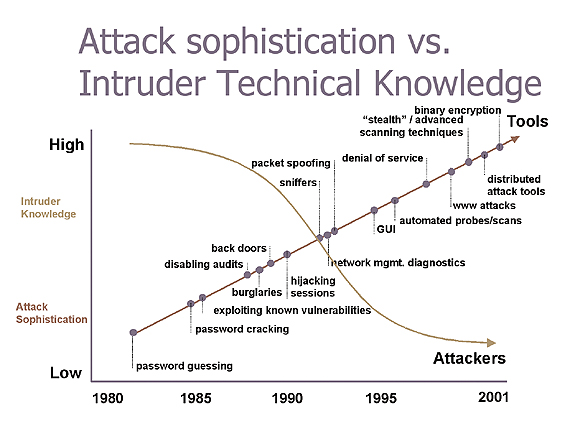
\includegraphics[width=12cm]{./images/AttackKnowledgeChart}
  \captionsource{Gegenüberstellung des benötigten Wissens und der Fähigkeiten der Angreifer}{\url{https://bizforum.aosoft.com/whitepapers/candle-4.htm}}
\end{figure}


\section{Täter-Typen}
Die Motive der Täter sind sehr unterschiedlich. Diese reichen von sozialen, politischen, finanziellen, staatlich-politischen Motiven über technische Ambitionen bis hin zu Regierungen oder Gruppierungen wie Anonymous. Neben der Motivation können die Täter auch nach Aussen- und Innentätern unterschieden werden. Innentäter verfügen über Insider-Wissen und arbeiten in der Regel für das angegriffene Unternehmen oder die angegriffene Organisation. Der Anteil an Innentätern am gesamten Tätervolumen ist sehr hoch und wächst stetig. Unternehmen und Organisationen sind sich dessen aber nicht immer bewusst und wähnen sich in falscher Sicherheit.

Die "`Berufsbezeichnungen"' der Täter sind sehr unterschiedlich und vielfältig. Nachfolgend sind einige der gängigsten Bezeichnungen und deren Bedeutung aufgelistet. Alle diese Berufsbezeichnungen stellen eine spezielle Ausprägung von Hackern dar. Hacker gibt es nicht nur im Informatik-Bereich, sondern auch in anderen Bereichen wo Technik allgegenwärtig ist. Hacker sind Personen, welche gezielt Schwachstellen (zum Beispiel in einem Computer-System) suchen und diese anschliessend ausnutzen. 

\begin{itemize}
\item \textbf{White-Hat oder "`Ethical-Hacker"' }\\
Ein White-Hat oder Ethical-Hacker führt seine Tätigkeiten nur mit ausdrücklicher Genehmigung durch und verhalten sich immer nach der Hackerethik. Sie sind meist in der Sicherheitsabteilung einer Organisation oder für eine spezialisierte Unternehmung im Security-Bereich tätig. Ihre Aufgabe ist es die Systeme und Netzwerke mit Penetrationstests zu prüfen, Schwachstellen zu finden und anschliessend entsprechende Massnahmen zu definieren.

\item \textbf{Black-Hats} \\
Black-Hats nutzen Schwachstellen in der Regel für die eigene Bereicherung oder zur Erlangung von Ansehen aus. Im Gegensatz zu White-Hats haben sie keine Genehmigung, um diese Aktivitäten durchzuführen, diese sind somit illegal und können von einer Strafverfolgungsbehörde verfolgt werden.

\item \textbf{Gray-Hats} \\
Gray-Hats bewegen sich zwischen den Welten von Black-Hats und White-Hats. Auch sie verschaffen sich unter Ausnutzung von Schwachstellen unautorisierten Zugang zu Computer-Systemen. Im Gegensatz zu Black-Hats verlassen Gray-Hats das System / Netzwerk wieder, sobald sie sich Zugang verschafft haben. Anschliessend benachrichtigen Sie den Besitzer oder Administrator des gehackten Systems, um diesen auf die Schwachstelle aufmerksam zu machen.

\item \textbf{Elite Hacker} \\
Elite Hacker ist nicht eine direkte Bezeichnung, sondern eher ein sozialer Status für sehr versierte / fähige Hacker.

\item \textbf{Script Kiddie} \\
Ein Script Kiddie hat im Gegensatz zu einem Black-Hat wenig bis gar kein fachliches Know-How und verwendet für seine Attacken vorwiegend vorgefertigte Tools und Scripts.
\end{itemize}


\section{Typischer Ablauf}
Ein Angriff kann in die nachfolgenden Phasen gegliedert werden. Diese können je nach Angriff in unterschiedlichen Ausprägungen vorkommen.

\subsection{Survey (Untersuchung)}
In dieser Phase werden so viele Informationen wie möglich gesammelt. Dazu gehören Informationen über die Organisation, die eingesetzte Hard- und Software und Prozesse. Anschliessend wird versucht so viele Schwachstellen wie möglich zu ermitteln. Zum einen wird ein Footprinting durchgeführt, welches so viele Informationen wie möglich über die Systeme zu Tage befördern soll. Zum Footprinting gehören unter anderem Port- und Protokollscanns und DNS- und WHOIS-Abfragen. Zum anderen werden mit Hilfe von Social Engeineering und Commodity-Toolkits und -Techniken weitere Schwachstellen ermittelt.


\subsection{Delivery (Positionierung)}
Diese Phase beschäftigt sich mit den expliziten Vorbereitungen für die Ausnutzung der Schwachstellen. Der Angreifer versucht das für dieses Szenario am besten geeignete Vorgehen zu ermitteln und bringt sich anschliessend in Position um die Schwachstellen auszunutzen. Eine typische Aktion in dieser Phase wäre zum Beispiel der Versand einer infizierten E-Mail oder das Unterjubeln eines infizierten USB-Sticks.


\subsection{Breach (Ausnutzung)}
In dieser Phase wird die Schwachstelle ausgenutzt, um dem Angreifer Zugang zum gewünschten System zu verschaffen.

\subsection{Affect (Beeinträchtigung / Infizierung)}
Nach dem der Angreifer Zugang zum System erlangt hat, unternimmt er weitere Schritte um sein eigentliches Ziel zu erreichen. Dies kann zum Beispiel die Erweiterung seiner Zugriffsrechte, die Einrichtung von Hintertüren, die Sammlung von Daten oder der Angriff eines weiteren Systems sein.


\subsection{Clean Up (Aufräumen)}
Je nach Ziel und Zweck des Angreifers verwischt er seine Spuren und räumt auf, damit er unerkannt bleibt oder allenfalls zu einem späteren Zeitpunkt nochmals zurückkehren kann.
